% Data flow diagram
% Author: David Fokkema
\documentclass{article}
\usepackage{tikz}
\usetikzlibrary{arrows}

% Defines a `datastore' shape for use in DFDs.  This inherits from a
% rectangle and only draws two horizontal lines.
\makeatletter
\pgfdeclareshape{datastore}{
  \inheritsavedanchors[from=rectangle]
  \inheritanchorborder[from=rectangle]
  \inheritanchor[from=rectangle]{center}
  \inheritanchor[from=rectangle]{base}
  \inheritanchor[from=rectangle]{north}
  \inheritanchor[from=rectangle]{north east}
  \inheritanchor[from=rectangle]{east}
  \inheritanchor[from=rectangle]{south east}
  \inheritanchor[from=rectangle]{south}
  \inheritanchor[from=rectangle]{south west}
  \inheritanchor[from=rectangle]{west}
  \inheritanchor[from=rectangle]{north west}
  \backgroundpath{
    %  store lower right in xa/ya and upper right in xb/yb
    \southwest \pgf@xa=\pgf@x \pgf@ya=\pgf@y
    \northeast \pgf@xb=\pgf@x \pgf@yb=\pgf@y
    \pgfpathmoveto{\pgfpoint{\pgf@xa}{\pgf@ya}}
    \pgfpathlineto{\pgfpoint{\pgf@xb}{\pgf@ya}}
    \pgfpathmoveto{\pgfpoint{\pgf@xa}{\pgf@yb}}
    \pgfpathlineto{\pgfpoint{\pgf@xb}{\pgf@yb}}
 }
}
\makeatother

\begin{document}
\begin{center}
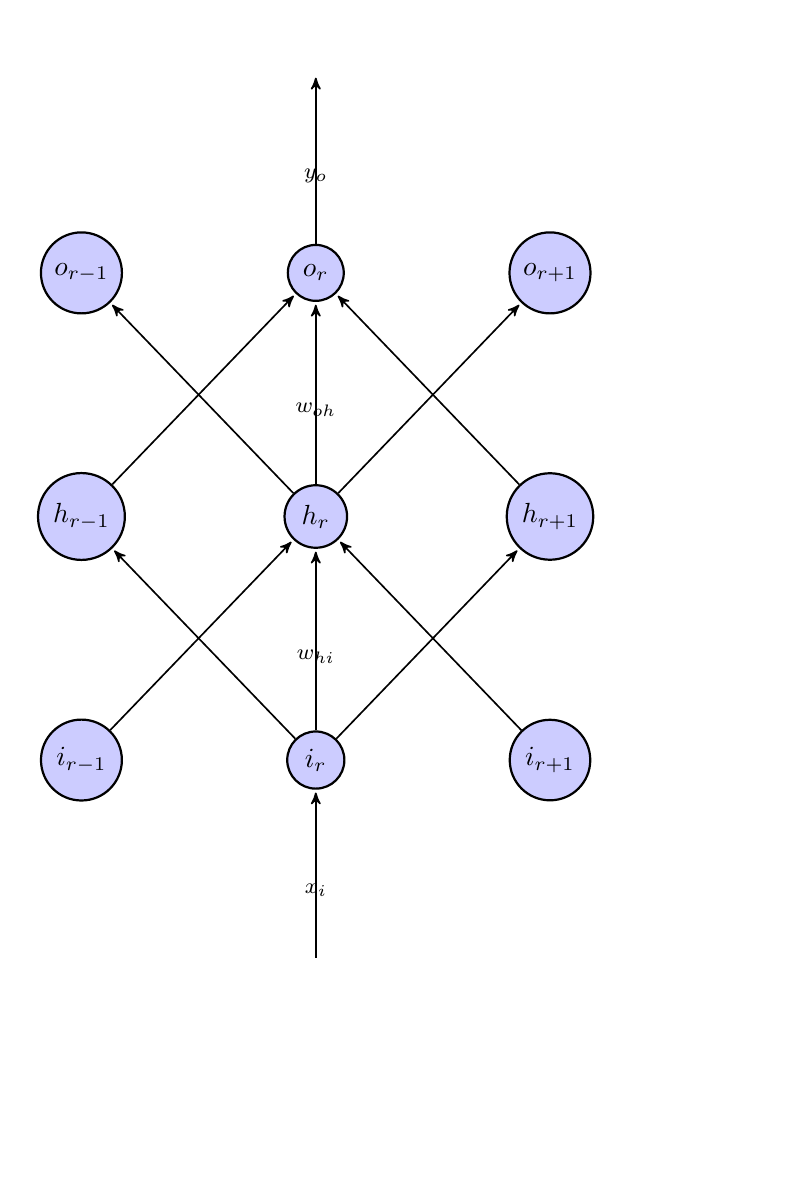
\begin{tikzpicture}[
  font=\sffamily,
  every matrix/.style={ampersand replacement=\&,column sep=2cm,row sep=2cm},
  source/.style={draw,thick,rounded corners,fill=yellow!20,inner sep=.3cm},
  process/.style={draw,thick,circle,fill=blue!20},
  sink/.style={source,fill=green!20},
  datastore/.style={draw,very thick,shape=datastore,inner sep=.3cm},
  dots/.style={gray,scale=2},
  to/.style={->,>=stealth',shorten >=1pt,semithick,font=\sffamily\footnotesize},
  every node/.style={align=center}]

  % Position the nodes using a matrix layout
  \matrix{
    \& \node[dots] (y2) {}; \&  \\

    \node[process] (o1) {$o_{r-1}$};
      \& \node[process] (o2) {$o_{r}$}; 
      \& \node[process] (o3) {$o_{r+1}$}; \& \\

    \node[process] (h1) {$h_{r-1}$};
      \& \node[process] (h2) {$h_{r}$}; 
      \& \node[process] (h3) {$h_{r+1}$}; \& \\

    \node[process] (i1) {$i_{r-1}$};
      \& \node[process] (i2) {$i_{r}$}; 
      \& \node[process] (i3) {$i_{r+1}$}; \\

	\& \node[dots] (x2) {}; \&  \\

  
    
      \\
  };

  % Draw the arrows between the nodes and label them.
  \draw[to] (h2) -- node[midway,below] {}  (o3);
  \draw[to] (h2) -- node[midway,below] {$w_{oh}$}  (o2);
  \draw[to] (h2) -- node[midway,below] {}  (o1);
  \draw[to] (h1) -- node[midway,above] {}  (o2);
  \draw[to] (h3) -- node[midway,above] {}  (o2);

  \draw[to] (i2) -- node[midway,below] {}  (h3);
  \draw[to] (i2) -- node[midway,below] {$w_{hi}$}  (h2);
  \draw[to] (i2) -- node[midway,below] {}  (h1);
  \draw[to] (i1) -- node[midway,above] {}  (h2);
  \draw[to] (i3) -- node[midway,above] {}  (h2);

  \draw[to] (x2) -- node[midway,below] {$x_{i}$} (i2);
\draw[to] (o2) -- node[midway,below] {$y_{o}$} (y2);


\end{tikzpicture}
\end{center}
\end{document}